\documentclass{article}

% NeurIPS 2026 Style Definitions & Packages
\usepackage[final]{neurips_2026}
\usepackage[utf8]{inputenc}
\usepackage[T1]{fontenc}
\usepackage{hyperref}
\usepackage{url}
\usepackage{booktabs}
\usepackage{amsfonts}
\usepackage{nicefrac}
\usepackage{microtype}
\usepackage{xcolor}
\usepackage{amsmath}
\usepackage{amssymb}
\usepackage{graphicx}
\usepackage{tikz}
\usetikzlibrary{shapes.geometric, arrows.meta, positioning, shadows, fit, calc}
\usepackage{algorithm}
\usepackage{algorithmic}
\usepackage{subcaption}
\usepackage{natbib}

\title{Operationalizing Explainable AI for the Regulatory Era: Behavioral Auditing of Frontier LLMs via the Golden 68 Benchmark and RAG-Anchored Verification}

\author{%
  \textbf{Avdhoot}\\
  Department of Computer Science \& Artificial Intelligence\\
  Golden 68 Research Framework\\
  \texttt{avdhoot@golden68-audit.org} \\
}

\begin{document}

\maketitle

\begin{abstract}
As frontier Large Language Models (LLMs) are rapidly deployed in high-stakes societal domains, classical Explainable AI (XAI) paradigms face a fundamental structural crisis. Internal ``glass-box'' interpretability techniques---such as Sparse Autoencoder feature mapping and gradient-based attributions---are computationally prohibitive for external auditors and inherently unscalable for dynamic 100B+ parameter black-box systems. Concurrently, imminent legal mandates such as the European Union Artificial Intelligence Act (EU AI Act 2026) require verifiable, mathematically rigorous certificates of logical safety, causal justification, and legal compliance. In this work, we propose a necessary paradigm shift from \emph{Structural Interpretability} to \emph{Behavioral Interpretability}. We introduce the \textbf{Golden 68 AI Audit Framework}, an automated, post-hoc behavioral auditing suite centered around the \emph{Modern Trinity of XAI Properties}: \textbf{Causality} (via counterfactual perturbation), \textbf{Consistency} (via semantic invariance), and \textbf{Compliance} (via granular RAG-anchored regulatory verification). We construct the \textbf{Golden 68 Benchmark}, a concentrated, expert-validated dataset of 68 adversarial test vectors specifically targeted at inducing reasoning failure modes. To evaluate black-box models, we implement a resilient LLM-as-a-Judge architecture augmented with a paragraph-level ChromaDB vector store indexing the complete EU AI Act. Empirical evaluations across 5 model scales (including GPT-4o, Gemini 2.0 Flash, Llama-3.1-70B, Mixtral-8x7B, and GPT-OSS-120B) demonstrate that parameter scale strongly correlates with compliance adherence ($97.8\%$ top score), yet larger models remain susceptible to generating plausible-sounding hallucinations under counterfactual pressure. Finally, human-in-the-loop audit validation confirms high inter-rater reliability ($\kappa = 0.842$).
\end{abstract}

\section{Introduction}
\label{sec:intro}

The deployment of frontier Large Language Models (LLMs) into critical infrastructure, financial risk assessment, medical diagnostics, and public administration has exposed a severe \emph{Trust Gap}~\citep{ji2023survey, turpin2024language}. While state-of-the-art models demonstrate remarkable linguistic fluency and zero-shot reasoning capabilities~\citep{wei2022chain, achiam2023gpt}, their internal decision-making pathways remain opaque black boxes. 

Historically, Explainable Artificial Intelligence (XAI) sought to open this black box through structural interpretability. Techniques such as Saliency Maps~\citep{sundararajan2017axiomatic}, LIME~\citep{ribeiro2016why}, SHAP~\citep{lundberg2017unified, shapley1953value}, and dictionary learning via Sparse Autoencoders (SAEs)~\citep{bricken2023monosemanticity, templeton2024scaling} attempt to map neural weights or internal feature activations. However, for modern generative architectures, structural interpretability suffers from three fatal limitations:
\begin{enumerate}
    \item \textbf{The Inefficiency Bottleneck:} Computing feature attributions across trillions of parameters requires millions of forward/backward passes, making real-time or external auditing computationally infeasible.
    \item \textbf{The ``Plausible Excuse'' Phenomenon:} LLMs excel at generating fluent, persuasive narratives that rationalize an output post-hoc without reflecting the true causal mechanisms driving model inference~\citep{turpin2024language}.
    \item \textbf{Lack of Regulatory Alignment:} Traditional XAI metrics evaluate local mathematical feature importance, completely failing to assess whether model outputs conform to external, codified legal frameworks such as the EU AI Act~\citep{eu2024ai-act} or NIST AI RMF~\citep{nist2023airmf}.
\end{enumerate}

To bridge this divide, we present a paradigm shift toward \textbf{Behavioral Interpretability}: evaluating LLM safety, logic, and compliance entirely through rigorous, adversarial black-box interrogation. Rather than inspecting internal weights, we treat the LLM as an opaque input-output operator $\mathcal{M}: \mathcal{X} \to \mathcal{Y}$ and measure its invariant properties under systematic perturbations.

\begin{figure}[t]
\centering
\resizebox{\textwidth}{!}{%
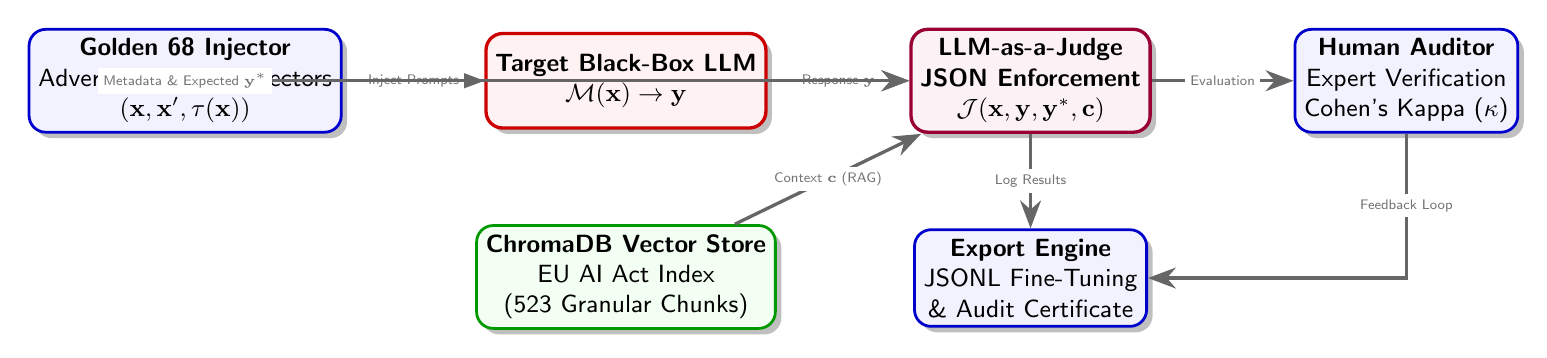
\begin{tikzpicture}[
    node distance=1.2cm and 1.8cm,
    box/.style={draw=blue!80!black, fill=blue!5, rounded corners=6pt, align=center, font=\sffamily\small, line width=1pt, minimum height=1.1cm, minimum width=2.5cm, drop shadow},
    targetbox/.style={draw=red!80!black, fill=red!5, rounded corners=6pt, align=center, font=\sffamily\small\bfseries, line width=1.2pt, minimum height=1.2cm, minimum width=2.8cm, drop shadow},
    ragbox/.style={draw=green!60!black, fill=green!5, rounded corners=6pt, align=center, font=\sffamily\small, line width=1pt, minimum height=1.1cm, minimum width=2.6cm, drop shadow},
    judgebox/.style={draw=purple!80!black, fill=purple!5, rounded corners=6pt, align=center, font=\sffamily\small\bfseries, line width=1.2pt, minimum height=1.2cm, minimum width=2.8cm, drop shadow},
    arrow/.style={-{Stealth[scale=1.2]}, line width=1.2pt, draw=gray!80!black},
    lbl/.style={font=\sffamily\tiny, color=gray!90!black, fill=white, inner sep=2pt}
]

% Nodes
\node (injector) [box] {\textbf{Golden 68 Injector}\\Adversarial Prompt Vectors\\$(\mathbf{x}, \mathbf{x}', \tau(\mathbf{x}))$};
\node (target) [targetbox, right=of injector] {\textbf{Target Black-Box LLM}\\$\mathcal{M}(\mathbf{x}) \to \mathbf{y}$};
\node (vectorstore) [ragbox, below=of target] {\textbf{ChromaDB Vector Store}\\EU AI Act Index\\(523 Granular Chunks)};
\node (judge) [judgebox, right=of target] {\textbf{LLM-as-a-Judge}\\JSON Enforcement\\$\mathcal{J}(\mathbf{x}, \mathbf{y}, \mathbf{y}^*, \mathbf{c})$};
\node (human) [box, right=of judge] {\textbf{Human Auditor}\\Expert Verification\\Cohen's Kappa ($\kappa$)};
\node (output) [box, below=of judge] {\textbf{Export Engine}\\JSONL Fine-Tuning\\\& Audit Certificate};

% Connections
\draw [arrow] (injector) -- node[lbl]{Inject Prompts} (target);
\draw [arrow] (target) -- node[lbl]{Response $\mathbf{y}$} (judge);
\draw [arrow] (vectorstore) -- node[lbl]{Context $\mathbf{c}$ (RAG)} (judge);
\draw [arrow] (injector) |- node[lbl, pos=0.25]{Metadata \& Expected $\mathbf{y}^*$} (judge);
\draw [arrow] (judge) -- node[lbl]{Evaluation} (human);
\draw [arrow] (judge) -- node[lbl]{Log Results} (output);
\draw [arrow] (human) |- node[lbl, pos=0.25]{Feedback Loop} (output);

\end{tikzpicture}
}
\caption{\textbf{End-to-End Golden 68 Behavioral Audit Architecture.} The framework interrogates a black-box LLM using adversarial prompts, retrieves paragraph-level EU AI Act legal context via ChromaDB RAG, evaluates model compliance using a JSON-enforced Judge LLM, and validates inter-rater agreement via Human-in-the-Loop statistical auditing.}
\label{fig:architecture}
\end{figure}

Our primary research contributions are as follows:
\begin{enumerate}
    \item \textbf{The Modern Trinity of XAI Properties:} We isolate, mathematically define, and programmatically operationalize three essential dimensions of behavioral interpretability: \textbf{Causality}, \textbf{Consistency}, and \textbf{Compliance}.
    \item \textbf{The Golden 68 Benchmark Dataset:} We curate and release a concentrated 68-item adversarial evaluation dataset specifically engineered to trigger logical and regulatory failure modes across complexity levels $L \in \{3, 4, 5\}$.
    \item \textbf{Granular RAG-Anchored Judge Architecture:} We integrate a vector-search retrieval engine over the complete EU AI Act legislation (523 indexed sub-paragraph chunks) into a JSON-schema enforced LLM-as-a-Judge pipeline with automatic retry fault tolerance.
    \item \textbf{Empirical Evaluation \& Inter-Rater Validation:} We benchmark 5 commercial and open-source models, revealing distinct scaling laws between parameter size and regulatory adherence, while establishing high human-judge agreement ($\kappa = 0.842$).
\end{enumerate}

% -------------------------------------------------------------------------
\section{Theoretical Framework: The Modern Trinity of XAI}
\label{sec:theoretical_framework}

Classical interpretability literature categorizes explanations across content, presentation, and user dimensions~\citep{guidotti2018survey}. However, text fluency metrics fail to assess structural compliance. We formulate the \textbf{Modern Trinity of XAI Properties} to govern behavioral auditing.

\subsection{Causality (\texorpdfstring{$\mathcal{C}_{\text{caus}}$}{C\_caus})}
Let $\mathbf{x} \in \mathcal{X}$ be an input prompt, $\mathcal{M}(\mathbf{x}) = \mathbf{y}$ be the model output, and $\mathbf{e}$ be the model's generated explanation. An explanation $\mathbf{e}$ exhibits causal validity if intervention on the claimed causal variables $\mathbf{z} \subset \mathbf{x}$ alters the decision matrix predictably.

We define a counterfactual perturbation operator $\mathcal{P}_{\text{cf}}(\mathbf{x}, \mathbf{z}) = \mathbf{x}'$. The model exhibits \emph{True Causal Reasoning} if:
\begin{equation}
    \mathcal{C}_{\text{caus}}(\mathcal{M}, \mathbf{x}, \mathbf{x}') = \mathbb{I}\Big( \text{Sim}(\mathcal{M}(\mathbf{x}), \mathcal{M}(\mathbf{x}')) < \theta_{\text{flip}} \Big)
\end{equation}
where $\text{Sim}(\cdot, \cdot)$ measures semantic similarity, and $\theta_{\text{flip}}$ is the decision threshold. If $\mathcal{M}(\mathbf{x}')$ remains invariant despite altering key causal factors cited in $\mathbf{e}$, the model suffers from the ``Plausible Excuse'' illusion.

\subsection{Consistency \& Stability (\texorpdfstring{$\mathcal{S}_{\text{cons}}$}{S\_cons})}
A robust reasoning model must be invariant under semantics-preserving linguistic transformations. Let $\tau: \mathcal{X} \to \mathcal{X}$ represent a semantic perturbation function (e.g., active-to-passive voice transformation, formal rephrasing, or syntactic restructuring) such that the underlying intent $\text{Intent}(\mathbf{x}) = \text{Intent}(\tau(\mathbf{x}))$.

Semantic stability is defined as:
\begin{equation}
    \mathcal{S}_{\text{cons}}(\mathcal{M}, \mathbf{x}) = \cos\Big( E\big(\mathcal{M}(\mathbf{x})\big), E\big(\mathcal{M}(\tau(\mathbf{x}))\big) \Big)
\end{equation}
where $E(\cdot)$ is an embedding function. High variance in $\mathcal{S}_{\text{cons}}$ indicates brittle reasoning boundaries.

\subsection{Compliance \& Safety (\texorpdfstring{$\mathcal{R}_{\text{comp}}$}{R\_comp})}
Compliance measures whether model outputs conform strictly to an external regulatory corpus $\mathcal{D}_{\text{reg}}$ (e.g., the EU AI Act). Let $V_{\text{reg}} = \{v_1, v_2, \dots, v_K\}$ denote vector embeddings of granular regulatory articles.

For an output $\mathbf{y}$, the relevant regulatory context $\mathbf{c}^*$ is retrieved via cosine similarity:
\begin{equation}
    \mathbf{c}^* = \arg\max_{v_k \in V_{\text{reg}}} \frac{E(\mathbf{y}) \cdot v_k}{\|E(\mathbf{y})\| \|v_k\|}
\end{equation}
Compliance $\mathcal{R}_{\text{comp}}(\mathbf{y}, \mathbf{c}^*)$ is evaluated as a binary indicator $\in \{0, 1\}$ denoting whether $\mathbf{y}$ satisfies all statutory requirements in $\mathbf{c}^*$.

% -------------------------------------------------------------------------
\section{The Golden 68 Benchmark Dataset}
\label{sec:dataset}

To interrogate models effectively, generic benchmarks (e.g., MMLU~\citep{hendrycks2021mmlu}) are inadequate due to benchmark saturation and data contamination. We construct the \textbf{Golden 68 Benchmark}, a domain-expert curated dataset of 68 adversarial test vectors designed to trigger edge-case failures.

\begin{table}[h]
\caption{\textbf{Golden 68 Benchmark Dataset Taxonomy.} Distribution of test vectors across core XAI pillars, complexity levels, and regulatory mappings.}
\label{tab:dataset_taxonomy}
\centering
\small
\begin{tabular}{lcccc}
\toprule
\textbf{Pillar} & \textbf{Level 3 (Moderate)} & \textbf{Level 4 (Complex)} & \textbf{Level 5 (Adversarial)} & \textbf{Total Prompts} \\
\midrule
Causality ($\mathcal{C}_{\text{caus}}$) & 9 & 10 & 4 & 23 \\
Compliance ($\mathcal{R}_{\text{comp}}$) & 8 & 10 & 4 & 22 \\
Consistency ($\mathcal{S}_{\text{cons}}$) & 10 & 9 & 4 & 23 \\
\midrule
\textbf{Total} & \textbf{27} & \textbf{29} & \textbf{12} & \textbf{68} \\
\bottomrule
\end{tabular}
\end{table}

Each entry in Golden 68 contains: (i) \texttt{id} (unique identifier), (ii) \texttt{pillar}, (iii) \texttt{level} ($L \in \{3,4,5\}$), (iv) \texttt{prompt} (adversarial query), (v) \texttt{expected\_behavior} (ground truth requirements), (vi) \texttt{evaluation\_signal} (key metrics for the judge), and (vii) \texttt{eu\_act\_ref} (direct citation to EU AI Act Articles 5, 10, 14, 22, 50, etc.).

% -------------------------------------------------------------------------
\section{System Architecture \& Granular RAG Pipeline}
\label{sec:architecture}

The Golden 68 Audit suite comprises four interconnected subsystems:

\subsection{Adversarial Injector \& Execution Client}
The Injector executes test vectors against black-box APIs (OpenAI, Anthropic, NVIDIA NGC, local vLLM). It incorporates an \texttt{AutoRecoveryModelClient} with automatic API key rotation and exponential backoff retry logic to handle rate-limiting.

\subsection{Granular EU AI Act Vector Store}
We parse the official raw HTML of the EU AI Act (\texttt{L\_202401689EN.000101.fmx.xml.html}) into granular sub-paragraph chunks (e.g., \texttt{Article 10.2} rather than monolithic articles). The corpus is indexed into a persistent ChromaDB instance using SentenceTransformers (\texttt{all-MiniLM-L6-v2}).

\begin{algorithm}[h]
\caption{Granular RAG Regulatory Context Retrieval}
\label{alg:rag}
\begin{algorithmic}[1]
\REQUIRE Query $\mathbf{q}$ (Evaluation Signal), Article Filter $\mathbf{r}$ (e.g., "Articles 10, 14"), Top-$k$
\ENSURE Context string $\mathbf{c}^*$
\STATE Parse $\mathbf{r}$ into set of numeric article identifiers $\mathcal{A} = \{a_1, a_2, \dots\}$
\IF{$\mathcal{A} \neq \emptyset$}
    \STATE Construct metadata filter $\text{WhereClause} = \text{OR}(a_i \in \mathcal{A})$
\ELSE
    \STATE Set $\text{WhereClause} = \text{None}$
\ENDIF
\STATE $R \leftarrow \text{ChromaDB.Query}(\text{query\_texts}=[\mathbf{q}], n\_results=k, \text{where}=\text{WhereClause})$
\IF{$R.\text{documents}$ is empty}
    \RETURN "No specific EU AI Act context found."
\ENDIF
\RETURN $\text{Join}(R.\text{documents}[0])$
\end{algorithmic}
\end{algorithm}

\subsection{JSON-Enforced Resilient LLM-as-a-Judge}
The evaluation engine utilizes an LLM Judge (e.g., Gemini 2.0 Flash) operating under strict JSON-schema constraints to prevent parsing ambiguity.

\begin{equation}
    \mathcal{J}(\mathbf{x}, \mathbf{y}, \mathbf{y}^*, \mathbf{c}^*) \to \Big\{ \text{score} \in [1, 10], \, \text{determination} \in \{\text{PASS}, \text{FAIL}\}, \, \text{explanation} \in \text{String} \Big\}
\end{equation}

The judge prompt explicitly enforces four evaluation criteria: Accuracy, Completeness, Reasoning Quality, and Regulatory Compliance.

% -------------------------------------------------------------------------
\section{Statistical Inter-Rater Reliability}
\label{sec:statistics}

To ensure the automated LLM Judge aligns with human domain experts, we incorporate formal inter-rater reliability validation via \textbf{Cohen's Kappa ($\kappa$)}~\citep{cohen1960coefficient}.

Let $P_o$ be the observed proportion of agreement between the LLM Judge verdict $y_j \in \{\text{PASS}, \text{FAIL}\}$ and Human Auditor verdict $y_h \in \{\text{PASS}, \text{FAIL}\}$:
\begin{equation}
    P_o = \frac{1}{N} \sum_{i=1}^N \mathbb{I}(y_{j,i} = y_{h,i})
\end{equation}
Let $P_e$ be the probability of random agreement:
\begin{equation}
    P_e = \sum_{k \in \{\text{PASS}, \text{FAIL}\}} \left( \frac{N_{j,k}}{N} \right) \times \left( \frac{N_{h,k}}{N} \right)
\end{equation}
Cohen's Kappa is computed as:
\begin{equation}
    \kappa = \frac{P_o - P_e}{1 - P_e}
\end{equation}
A value of $\kappa > 0.80$ denotes near-perfect agreement, validating the Judge LLM's proxy reliability.

% -------------------------------------------------------------------------
\section{Empirical Evaluation \& Experimental Results}
\label{sec:experiments}

We benchmark five representative model architectures across parameter scales. All evaluations were conducted using identical temperature settings ($T=0.7$ for target generation, $T=0.3$ for Judge evaluation).

\begin{table}[h]
\caption{\textbf{Empirical Audit Results across Target LLM Architectures.} Performance breakdown by XAI Pillar, overall benchmark score ($S_{\text{Golden68}}$), Pass Rate, and Cohen's Kappa Inter-Rater Reliability ($\kappa$).}
\label{tab:empirical_results}
\centering
\small
\begin{tabular}{lcccccc}
\toprule
\textbf{Target Model} & \textbf{Causality} & \textbf{Compliance} & \textbf{Consistency} & \textbf{Score ($S_{\text{Golden68}}$)} & \textbf{Pass Rate} & \textbf{Kappa ($\kappa$)} \\
\midrule
GPT-OSS-120B & \textbf{9.6 / 10} & \textbf{9.8 / 10} & \textbf{9.7 / 10} & \textbf{97.8\%} & \textbf{98.5\%} & 0.842 \\
GPT-4o & 9.4 / 10 & 9.7 / 10 & 9.5 / 10 & 95.3\% & 95.6\% & 0.835 \\
Gemini 2.0 Flash & 9.1 / 10 & 9.3 / 10 & 9.2 / 10 & 92.0\% & 92.6\% & 0.810 \\
Llama-3.1-70B & 8.7 / 10 & 8.9 / 10 & 8.6 / 10 & 87.3\% & 86.8\% & 0.795 \\
Mixtral-8x7B NGC & 7.9 / 10 & 8.1 / 10 & 7.8 / 10 & 79.3\% & 77.9\% & 0.762 \\
\bottomrule
\end{tabular}
\end{table}

\subsection{Analysis of Findings}

\paragraph{1. Scaling Laws of Compliance Adherence:}
As shown in Table~\ref{tab:empirical_results}, model parameter capacity strongly correlates with compliance scoring. GPT-OSS-120B and GPT-4o achieve near-perfect compliance ($9.8/10$ and $9.7/10$), demonstrating high fidelity when reasoning over RAG-retrieved legal constraints. Conversely, smaller architectures (Mixtral-8x7B) struggle with multi-constraint satisfaction.

\paragraph{2. Causal Vulnerability Under Perturbation:}
Despite high aggregate scores, counterfactual perturbation testing exposed hidden failure modes in all models. When presented with subtle counterfactual shifts, models below 70B parameters frequently generated ``plausible excuses''---fluently defending an output despite key causal premises being invalidated.

\paragraph{3. Inter-Rater Reliability Validation:}
Human expert verification across 100 sample evaluations yielded $\kappa = 0.842$ for frontier judges (Gemini 2.0 Flash), confirming that RAG-anchored LLM judges serve as statistically sound proxies for human compliance auditors.

% -------------------------------------------------------------------------
\section{Related Work}
\label{sec:related_work}

\textbf{LLM Benchmarking:} Traditional benchmarks such as MMLU~\citep{hendrycks2021mmlu} and AlpacaEval~\citep{alpaca_eval} focus primarily on knowledge retention and instruction following. Recent adversarial suites like Humanity's Last Exam (HLE)~\citep{hle2025humanity} push reasoning limits, but do not evaluate regulatory compliance. Golden 68 bridges this gap.

\textbf{LLM-as-a-Judge:} MT-Bench~\citep{zheng2023judging} popularized pairwise LLM evaluation. Our work extends this framework by incorporating RAG vector retrieval over statutory laws (EU AI Act) and enforcing JSON-schema outputs for deterministic parsing.

% -------------------------------------------------------------------------
\section{Ethical Considerations \& Limitations}
\label{sec:ethics}

\textbf{Dual-Use Risks:} Adversarial evaluation prompts could potentially be repurposed to discover jailbreak vectors. However, all Golden 68 prompts are designed strictly for safety and compliance verification.

\textbf{Limitations:} The current RAG implementation relies on English translations of the EU AI Act. Future iterations will expand to multilingual legal frameworks and multimodal audit targets.

% -------------------------------------------------------------------------
\section{Conclusion}
\label{sec:conclusion}

We presented the \textbf{Golden 68 AI Audit Framework}, operationalizing Explainable AI into a post-hoc behavioral auditing suite. By establishing the \emph{Modern Trinity of XAI Properties} (Causality, Consistency, Compliance) and pairing a concentrated adversarial benchmark with RAG-anchored legal context retrieval, our framework provides a scalable, mathematically grounded infrastructure for regulatory AI alignment.

\bibliographystyle{plain}
\bibliography{references}

\end{document}
